\chapter{IMPLEMENTASI}
Setelah melewati proses perancangan mengenai sistem yang akan dibuat, maka akan dilakukan implementasi dari sistem tersebut. Bab ini akan membahas mengenai implementasi dari sistem yang meliputi proses pembuatan setiap komponen sehingga sistem dapat berjalan dengan baik. Masing-masing proses pembuat komponen akan dilengkapi dengan \textit{pseudocode} atau konfigurasi dari sistem.  
\section{Lingkungan Implementasi}
  	Dalam mengimplementasikan sistem, digunakan beberapa perangkat pendukung sebagai berikut.
    \subsection{Perangkat Keras}
    Perangkat keras yang digunakan dalam pengembangan sistem adalah sebagai berikut:
    \begin{enumerate}
    \item Komputer dengan \textit{processor} Intel(R) Core(TM) i5-2120 CPU @ 3.30GHz dan RAM 8GB
    \item Dua Komputer dengan \textit{processor} Intel(R) Core(TM)2 Duo CPU E7200 @ 2.53GHz dan RAM 1GB
    \end{enumerate}
    \subsection{Perangkat Lunak}
    Perangkat lunak yang digunakan dalam pengembangan sistem adalah sebagai berikut:
    \begin{enumerate}
    \item Sistem Operasi Linux Mint 18.03 64 Bit sebagai \textit{docker host}.
    \item Sistem Operasi Ubuntu 14.04 LTS 64 Bit sebagai \textit{client}.
    \item Sistem Operasi Ubuntu Server 16.04 LTS 64 Bit sebagai \textit{server login}.
    \item \textit{Python} versi 3.5.2 untuk pengembangan web service. 
    \item \textit{Flask} versi 1.0.2 sebagai kerangka kerja \textit{Python}.
    \item \textit{Gunicorn} versi 19.8.1
    \item \textit{Supervisor} versi 3.2.0
    \item \textit{Nginx} versi 1.10.3
    \item \textit{Mitmproxy} versi 3.0.4 untuk mencatat semua \textit{traffic} dari \textit{client}.
    \item MySQL versi 5.7.18 untuk Sistem Manajemen Basis Data.
    \item \textit{Docker} versi 1.13.1 sebagai kontainer yang akan di pasangkan pada \textit{server}.
    \item \textit{Iptables} versi 1.6.0 untuk membuat aturan terhadap \textit{client}.
    \item \textit{Laravel} versi 5.4 sebagai kerangka kerja untuk halaman \textit{administrator}. 
    \item \textit{VIM} versi 7.4.1 sebagai \textit{text editor}.
    \end{enumerate}
    
  \section{Implementasi Pembuatan Halaman \textit{Login} dari Sebuah Sistem}
  Halaman \textit{login} dibangun pada sebuah \textit{server} dengan IP \texttt{10.151.36.173} dengan menggunakan sistem operasi Ubuntu Server 16.04 LTS 64 Bit. Pada implementasi pembuatan halaman \textit{login} dari sebuah sistem menggunakan perangkat lunak antara lain:
  \begin{enumerate}
  \item \textit{Python} versi 3.5.2.
  \item \textit{Flask} versi 1.0.2.
  \item \textit{Gunicorn} versi 19.8.1.
  \item \textit{Supervisor} versi 3.2.0.
  \item \textit{Nginx} versi 1.10.3.
  \end{enumerate}

  Lalu sistem operasi yang digunakan adalah sistem operasi Ubuntu Server 16.04 LTS 64 Bit, yang akan dipasang pada \textit{virtual machine} di \textit{Proxmox}. \textit{Python} akan berfungsi sebagai komponen dasar pembangunan sistem yang akan dibangun dengan menggunakan kerangka kerja \textit{Flask} dan dijalankan dengan \textit{Gunicorn} pada \textit{server} dengan IP \texttt{10.151.36.173} dengan \textit{port} 4000. Lalu \textit{Supervisor} akan berfungsi sebagai sebuah \textit{service} yang akan selalu menajalankan \textit{Gunicorn}. Sedangkan \textit{Nginx} akan berfungsi sebagai \textit{web server} untuk perangkat lunak halaman \textit{login} yang dijalankan oleh \textit{Gunicorn} pada \textit{server} dengan IP \texttt{10.151.36.173} dengan \textit{port} 4000 supaya bisa diakses oleh \textit{client}. Implementasi pembuatan halaman \textit{login} dari sebuah sistem akan terbagi menjadi implementasi \textit{web service} dan implementasi basis data.
  
  \subsection{Implementasi \textit{Web Service} pada Halaman \textit{Login}}
  Diperlukan beberapa tahap, antara lain pemasangan perangkat lunak dan tahap konfigurasi. Tahap pemasangan perangkat lunak dan tahap konfigurasi pada \textit{server} untuk halaman \textit{login} dijelaskan pada Lampiran A. 
  
  Perlu diperhatikan ketika menambahkan atau mengubah konfigurasi \textit{Supervisor} pada \texttt{/etc/supervisor/conf.d/} di \textit{server} untuk halaman \textit{login}, perlu dilakukan \textit{reload Supervisor} dengan menjalankan \textit{command} pada terminal seperti pada Kode Sumber \ref{reloadsupervisor}.\\ 
  \begin{minipage}{\linewidth}
  \begin{lstlisting}[caption=Command untuk Reload Supervisor,language=Python,label=reloadsupervisor]
  sudo supervisorctl reread
  sudo supervisorctl reload
  sudo supervisorctl status
  \end{lstlisting}
  \end{minipage}

  Perlu diperhatikan pula ketika menambahkan atau mengubah konfigurasi \textit{Nginx} pada \texttt{/etc/nginx/sites-available/} di \textit{server} untuk halaman \textit{login}, perlu dilakukan aktifasi konfigurasi \textit{Nginx} dengan menjalankan \textit{command} pada terminal seperti pada Kode Sumber \ref{aktifasikonfigurasinginx}.\\
  \begin{minipage}{\linewidth}
  \begin{lstlisting}[caption=Command untuk mengaktifkan konfigurasi Nginx,language=Python,label=aktifasikonfigurasinginx]
  sudo ln -s /etc/nginx/sites-available/app 
    /etc/nginx/sites-enabled/app
  \end{lstlisting}
  \end{minipage}
  Setelah itu, jalankan Kode Sumber \ref{restartnginx} supaya konfigurasi yang baru saja diaktifkan dapat digunakan.\\
  \begin{minipage}{\linewidth}
  \begin{lstlisting}[caption=Command untuk merestart Nginx,language=Python,label=restartnginx]
  sudo service nginx restart
  \end{lstlisting}
  \end{minipage}
  
  \subsubsection{Implementasi Tampilan Antarmuka Halaman \textit{Login}}
  Halaman \textit{login} merupakan halaman utama yang menampilkan sebuah \textit{form input} untuk \textit{client}. Pada halaman ini terdapat dua \textit{form input}, yaitu \textit{form input} untuk \texttt{Username} atau NRP dari \textit{client} dan juga \textit{form input} untuk \texttt{Password} dari \textit{client}. Implementasi antarmuka halaman \textit{login} dapat dilihat pada Gambar \ref{implementasihalamanlogin}.
  
\begin{figure}[H]
	\centering
	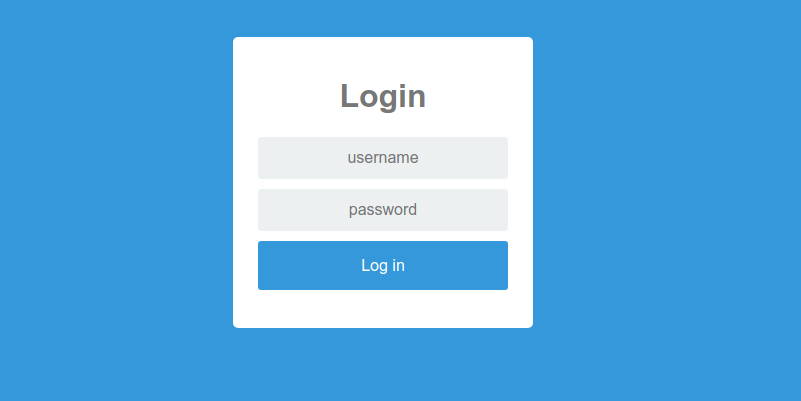
\includegraphics[width=\linewidth]{images/bab4/halamanlogin}
	\caption{Halaman \textit{Login}}
	\label{implementasihalamanlogin}
\end{figure}
  
  \subsubsection{Rute \textit{Web Service} pada Halaman \textit{Login}}
  Pada halaman \textit{login} diperlukan adanya rute-rute yang bisa diakses untuk melayani \textit{client}, supaya \textit{client} dapat membuka tampilan antar muka dari halaman \textit{login} dan juga supaya \textit{client} dapat mengirimkan permintaan untuk membuat kontainer \textit{docker} pada \textit{docker host}. Daftar rute yang disediakan oleh halaman \textit{loign} tertera pada Tabel \ref{tabelRuteWebServiceHalamnLogin}.\\
  \begin{longtable}{|p{0.15\textwidth}|p{0.25\textwidth}|p{0.4\textwidth}|p{0.3\textwidth}|} % L = Rata kiri untuk setiap kolom, | = garis batas vertikal.
  	
  	% Kepala tabel, berulang di setiap halaman
  	\caption{Daftar Rute \textit{Web Service}} \label{tabelRuteWebServiceHalamnLogin} \\
  	\hline
  	\textbf{HTTP Method} & \textbf{Rute} & \textbf{Deskripsi} \\ \hline
  	
  	\endfirsthead
  	\caption[]{Daftar Rute \textit{Web Service}}  \\
  	\hline
  	\textbf{HTTP Method} & \textbf{Rute} & \textbf{Deskripsi}  \\ \hline
  	
  	\endhead
  	\endfoot
  	\endlastfoot
  	
  	% Isi Tabel
  	GET & / & Berfungsi untuk mengarahkan \textit{redirect} ke rute \textit{login} dengan \textit{method} GET.\\ \hline
  	GET & /login & Berfungsi untuk menampilkan tampilan grafis antar muka halaman \textit{login} ketika \textit{client} belum \textit{login} ke dalam sistem dan untuk menampilkan tampilan grafis antar muka halaman sukses \textit{login} ketika \textit{client} telah berasil \textit{login} ke dalam sistem.\\ \hline
  	POST & /login & Berfungsi untuk menyimpan data hasil \textit{input} dari \textit{client} dan mengirimkan perintah untuk membuat kontainer \textit{docker} yang berisikan \textit{mitmproxy} secara otomatis pada \textit{docker host}.\\ \hline
  \end{longtable}
  
  \subsubsection{\textit{Pseduocode Web Service} pada Halaman \textit{Login}}
  Ketika \textit{client} belum \textit{login} ke dalam sistem, maka akan diarahkan ke tampilan grafis antar muka dari halaman \textit{login}. Lalu setelah \textit{client} berhasil \textit{login} ke dalam sistem, maka akan diarahkan ke tampilan grafis antar muka halaman sukses \textit{login}. Pada Kode Sumber \ref{pseudocodehalamanlogin} diperlihatkan bagaimana implementasinya dalam bentuk \textit{pseduocode}.
  
  \begin{minipage}{\linewidth}  
  \begin{lstlisting}[numbers=left, frame=single,tabsize=2,breaklines,caption={Pseudocode Web Service},label=pseudocodehalamanlogin]
  Check whether the client is already login or not yet
  	
  if session.get login
	  open welcome page
  else
	  open login page
	  if login success
			session.get login = True	  
  return  	
  \end{lstlisting}
  \end{minipage}
  
  
  \subsection{Implementasi Basis Data pada Halaman \textit{Login}}
  Berdasarkan hasil desain dan perancangan basis data pada bab 3 terdapat satu entitas yang diimplementasikan menjadi suatu tabel pada basis data MySQL, yaitu entitas \texttt{nrp-mahasiswa}. Detail implementasi \textit{query} untuk membuat basis data dengan entitas \texttt{nrp-mahasiswa} seperti pada Kode Sumber \ref{entitasnrpmahasiswa}.\\
  \begin{minipage}{\linewidth}
  \begin{lstlisting}[language=python, caption=\textit{Query} untuk membuat tabel testing,label=entitasnrpmahasiswa]
  CREATE TABLE nrp-mahasiswa (
	  id int(11) PRIMARY KEY AUTO_INCREMENT,
	  nrp VARCHAR(50)
	  password VARCHAR(50)
	  isLogin int(11)
  );
  \end{lstlisting}
  \end{minipage}
    
  \section{Implementasi Pembuatan Aturan untuk Mengarahkan \textit{Traffic Client} ke Halaman \textit{Login} dari Sistem}
  Pada implementasi pembuatan aturan untuk mengarahkan \textit{traffic client} ke halaman \textit{login} dari sistem diasumsikan bahwa belum ada \textit{client} yang telah \textit{login} ke dalam sistem. Karena diasumsikan bahwa belum ada \textit{client} yang telah berhasil \textit{login} ke dalam sistem, maka semua \textit{client} tidak diperbolehkan untuk mengakses internet. Kemudian untuk mengarahkan \textit{traffic} dari \textit{client} dibuatkan beberapa \textit{rules} dengan menggunakan \textit{iptables} pada \textit{Docker Host} dengan IP \texttt{10.151.36.134}. seperti Kode Sumber \ref{iptablesbeforelogin}. \\
  \begin{minipage}{\linewidth}
  	\begin{lstlisting}[caption=Command untuk mengarahkan \textit{client} ke halaman \textit{login},language=Python,label=iptablesbeforelogin]
  	iptables -I FORWARD 1 -s 192.168.99.0/24 -j REJECT
  	iptables -I FORWARD 1 -s 192.168.99.0/24 -p tcp d 10.151.36.173
  	--dport 4000 -j ACCEPT
  	iptables -t nat -I PREROUTING 1 -p tcp -s 192.168.99.0/24
  	--dport 80 -j DNAT --to 10.151.36.173:4000
  	\end{lstlisting}
  \end{minipage}  
  \indent \textit{Rules} pertama berfungsi untuk melarang semua \textit{client} untuk melewati \textit{router}. \textit{Rules} kedua berfungsi untuk mengizinkan semua \textit{client} membuka halaman \textit{login}. Sedangkan \textit{rules} ketiga berfungsi untuk mengarahkan semua \textit{traffic client} ke halaman \textit{login}.
	
  \section{Implementasi Pembuatan \textit{Middleware}}
  \textit{Middleware} dibangun pada \textit{Docker Host} dengan IP \texttt{10.151.36.134} dengan menggunakan sistem operasi Linux Mint 18.03 64 Bit. \textit{Middleware} merupakan komponen yang akan menerima permintaan dari \textit{client}, mengirimkan perintah untuk membuat kontainer \textit{docker} secara otomatis pada \textit{docker host}, dan menentukan rute \textit{traffic} dari \textit{client} menuju ke internet sesuai kontainer \textit{docker} masing-masing user. Implementasi \textit{middleware} akan terbagi menjadi implementasi basis data dan implementasi \textit{web service}.
  
  Pada implementasi pembuatan \textit{middleware} menggunakan perangkat unak antara lain:
  \begin{enumerate}
	\item \textit{Python} versi 3.5.2.
	\item \textit{Flask} versi 1.0.2.
	\item \textit{Docker} versi 1.13.1.
  \end{enumerate}
  
  \textit{Python} akan berfungsi sebagai komponen dasar pembangunan sistem, salah satunya adalah sebagai komponen dasar pembuatan \textit{middleware}, sedangkan \textit{Flask} akan berfungsi sebagai kerangka kerja untuk pembuatan \textit{middleware}. Implementasi pembuatan \textit{middleware} akan terbagi menjadi implementasi \textit{web service} dan implementasi basis data dan.
  
  \subsection{Implementasi \textit{Web Service} pada \textit{Middleware}}
  Diperlukan beberapa tahap, antara lain pemasangan perangkat lunak dan tahap konfigurasi. Tahap pemasangan perangkat lunak dan tahap konfigurasi pada \textit{middleware} di \textit{Docker Host} dijelaskan pada Lampiran B.
   
  Perlu diperhatikan supaya \textit{docker} dapat dijalankan ketika \textit{docker host} menyala, jalankan Kode Sumber \ref{systemctldocker}.\\
  \begin{minipage}{\linewidth}
  \begin{lstlisting}[caption=Command untuk installasi Flask,language=Python,label=systemctldocker]
  sudo systemctl enable docker
  \end{lstlisting}
  \end{minipage} 

  \subsubsection{Rute \textit{Web Service} pada \textit{Maaiddleware}}
  \textit{Middleware} tidak memiliki antar muka grafis. Namun tetap diperlukan adanya rute-rute yang bisa diakses untuk melayani permintaan penyediaan kontainer \textit{docker} dari \textit{client}. Daftar rute yang disediakan oleh \textit{middleware} tertera pada Tabel \ref{tabelRuteWebServiceDockerHost}.\\
  \begin{longtable}{|p{0.15\textwidth}|p{0.25\textwidth}|p{0.4\textwidth}|p{0.3\textwidth}|} % L = Rata kiri untuk setiap kolom, | = garis batas vertikal.
  	
  	% Kepala tabel, berulang di setiap halaman
  	\caption{Daftar Rute \textit{Web Service}} \label{tabelRuteWebServiceDockerHost} \\
  	\hline
  	\textbf{HTTP Method} & \textbf{Rute} & \textbf{Deskripsi} \\ \hline
  	
  	\endfirsthead
  	\caption[]{Daftar Rute \textit{Web Service}}  \\
  	\hline
  	\textbf{HTTP Method} & \textbf{Rute} & \textbf{Deskripsi}  \\ \hline
  	
  	\endhead
  	\endfoot
  	\endlastfoot
  	
  	% Isi Tabel
  	POST & /test/endpoint/ & Berfungsi untuk menyimpan data hasil \textit{input} dari \textit{client} dan mengirimkan perintah untuk membuat kontainer \textit{docker} yang berisikan \textit{mitmproxy} secara otomatis pada \textit{docker host}.\\ \hline
  \end{longtable}
  
  \subsubsection{\textit{Pseduocode Web Service} pada \textit{Middleware}}
  Saat \textit{client} telah memasukkan \textit{input} ke sistem, sistem akan mencocokkan terlebih dahulu dengan basis data \texttt{kontainer}. Jika benar, maka sistem akan mengirimkan data \textit{input} dari \textit{client} ke \textit{middleware}. Lalu \textit{middleware} akan menyimpan data \textit{input} dari \textit{client} ke dalam sebuah \textit{file}. Setelah itu \textit{middleware} akan mengirimkan perintah untuk membuat sebuah kontainer \textit{docker} yang berisikan \textit{mitmproxy} pada \textit{docker host}.
  
  Saat \textit{middleware} menyimpan data \textit{input} dari \textit{client} ke dalam sebuah \textit{file}, yang disimpan adalah \textit{username} atau NRP, \textit{IP Address}, dan \textit{port}. Nantinya \textit{port} tersebut akan menjadi \textit{port} khusus untuk kontainer \textit{docker} yang berisikan \textit{mitmproxy} untuk \textit{client} tersebut.
  
  Saat kontainer \textit{docker} yang berisikan \textit{mitmproxy} akan dibuat pada \textit{docker host}, sistem akan membuat kontainer \textit{docker} dengan \textit{mode network}=\textit{host}, nama sesuai \textit{IP Address} dari \textit{client} tersebut, dan \textit{port} kontainer \textit{docker} sesuai dengan \textit{port} yang sudah disimpan pada \textit{file}.
  
  Setelah kontainer \textit{docker} yang berisikan \textit{mitmproxy} berhasil dibuat, maka sistem akan membuat \textit{rules} yang berfungsi untuk mengarahkan \textit{traffic} dari \textit{client} menuju ke kontainer \textit{docker} milik \textit{client} tersebut, dan memperbolehkan \textit{client} untuk mengakses internet. Pada Kode Sumber \ref{pseudocodeoing} diperlihatkan bagaimana implementasinya dalam bentuk \textit{pseduocode}.
  \newline
  \begin{minipage}{\linewidth}  
  	\begin{lstlisting}[numbers=left, frame=single,tabsize=2,breaklines,caption={Pseudocode Web Service},label=pseudocodeoing]
  	Check whether the client is already login or not yet
  	
  	if session.get login
	  	create container
	  	add new rules to container
	  	return
  	else
	  	add new rules
	  	client open page login
	  	client login
	  	return  	
  	\end{lstlisting}
  \end{minipage}
  
  \subsection{Implementasi Basis Data pada \textit{Middleware}}
  Berdasarkan hasil perancangan basis data pada bab 3 terdapat 2 entitas yang diimplementasikan menjadi suatu tabel pada basis data MySQL, yaitu entitas \texttt{kontainer}. Detail implementasi entitas \texttt{kontainer} tertera pada Kode Sumber \ref{entitastesting}.
  \newline
  \begin{minipage}{\linewidth}
  \begin{lstlisting}[language=python, caption=\textit{Query} untuk membuat tabel testing,label=entitastesting]
  CREATE TABLE kontainer (
	  id int(11) PRIMARY KEY AUTO_INCREMENT,
	  username VARCHAR(50)
	  ip VARCHAR(50)
	  createdAt DATETIME
  );
  \end{lstlisting}
  \end{minipage}
    
  \section{Implementasi Pemasangan Kontainer \textit{Docker} pada \textit{Docker Host}}
  Setelah berhasil melakukan pemasangan \textit{docker} versi 1.13.1, sekarang lakukan konfigurasi supaya \textit{docker} tidak hanya dapat digunakan oleh \textit{root user} dari sebuah sistem. Hal ini dapat dilakukan dengan menjalankan perintah pada Kode Sumber \ref{konfigurasildocker1}.
  \newline
    \begin{minipage}{\linewidth}
	\begin{lstlisting}[caption=Perintah untuk installasi Ansible,language=Python,label=konfigurasildocker1]
	sudo groupadd docker
	sudo usermod -aG docker $USER
	\end{lstlisting}
	\end{minipage}
	
  \subsection{Menambahkan dan Memperbarui Kontainer \textit{Docker} yang Berisikan Mitmproxy}
  Setelah berhasil melakukan pemasangan \textit{docker} pada \textit{docker host} dan melakukan konfigurasi supaya \textit{docker} tidak hanya dapat digunakan oleh \textit{root user} dari sebuah sistem, selanjutnya dapat mencoba membuat sebuah kontainer \textit{docker} yang berisi aplikasi \textit{mitmproxy}. Untuk membuat sebuah kontainer \textit{docker} yang berisi \textit{mitmproxy}, penulis melakukannya dengan sistem operasi Ubuntu dalam format \textit{docker} yang disediakan oleh Docker Hub. Untuk melakukan unduh, jalankan perintah berikut pada Kode Sumber \ref{pullubuntu}.
  \newline
  \begin{minipage}{\linewidth}
  \begin{lstlisting}[caption=Perintah untuk \textit{Pull} Ubuntu,language=Python,label=pullubuntu]
  docker pull ubuntu
  \end{lstlisting}
  \end{minipage}
  Setelah berhasil diunduh, selanjutnya jalankan sistem operasi Ubuntu dengan menggunakan perintah yang tertera pada Kode Sumber \ref{runubuntu}.
  \newline
  \begin{minipage}{\linewidth}
  \begin{lstlisting}[caption=Perintah untuk Menjalankan \textit{Image} Ubuntu,language=Python,label=runubuntu]
  docker run --name testmitmproxy --privileged=True 
 	  --network=host ubuntu
  \end{lstlisting}
  \end{minipage}
	Parameter \texttt{--name} berguna untuk memberikan nama pada kontainer \textit{docker} agar mudah dikenali dimana lokasi aplikasi saat dijalankan. Pada kasus ini kontainer \textit{docker} diberi nama dengan \texttt{testmitmproxy}. Parameter \texttt{--privileged=True} berguna untuk memberikan kendali hak akses penuh kepada kontainer \textit{docker} tersebut, sama seperti dengan \textit{root user}. Parameter \texttt{--network=host} berguna untuk mendefinisikan jaringan yang akan digunakan oleh kontainer \textit{docker} tersebut. Setelah menjalankannya, kontainer \textit{docker} yang terbentuk dapat digunakan lebih lanjut, misalnya dengan mengubah data yang ada didalamnya, menambahkan fitur baru, atau hanya sekedar mengganti nama dari aplikasi.\\
	\indent Dalam kasus ini penulis menambahkan fitur baru, yaitu menambah \textit{mitmproxy}. Untuk menambah atau memasang \textit{mitmproxy} pada kontainer \textit{docker} yang baru saja dibuat, jalankan perintah berikut pada Kode Sumber \ref{installmitmproxy}.
	\newline
	\begin{minipage}{\linewidth}
	\begin{lstlisting}[caption=Perintah untuk Pemasangan \textit{Mitmproxy},language=Python,label=installmitmproxy]
	sudo apt-get update
	sudo apt-get install python3 python3-dev python3-pip
	sudo pip3 install cryptography
	sudo pip3 install mitmproxy
	\end{lstlisting}
	\end{minipage}
	
	\textit{Mitmproxy} versi 3.0.4 membutuhkan \textit{Python} minimal versi 3.5, maka dari itu penulis memasang \textit{Python} versi 3.5.2. \textit{Mitmproxy} juga membutuhkan modul \textit{cryptography} yang berguna untuk melakukan enkripsi maupun dekripsi ketika \textit{mitmproxy} sedang berjalan. Lalu aktifkan \texttt{ipv4.forwarding} dengan menjalankan perintah pada Kode Sumber \ref{ipv4forwarding}\\
	\newline
	\begin{minipage}{\linewidth}
	\begin{lstlisting}[caption=Perintah untuk Mengaktifkan \textit{ipv4.forwarding},language=Python,label=ipv4forwarding]
  sudo sysctl -w net.ipv4.ip_forward=1
	\end{lstlisting}
	\end{minipage}
	\indent Setelah berhasil melakukan pemasangan \textit{mitmproxy} pada kontainer \textit{docker}, jika ingin membuat \textit{images} baru dari kontainer \textit{docker} tersebut, maka hal pertama yang harus dilakukan adalah menghentikan kontainer \textit{docker} yang sedang berjalan dengan menggunakan perintah seperti pada Kode Sumber \ref{dockerstop}.
	\newline
	\begin{minipage}{\linewidth}
	\begin{lstlisting}[caption=Perintah untuk Menghentikan Kontainer \textit{Docker},language=Python,label=dockerstop]
	docker stop [nama_container]
	\end{lstlisting}
	\end{minipage}
	Nama \textit{container} ini tergantung dari nama kontainer \textit{docker} yang sudah dibuat. Untuk kasus yang digunakan oleh penulis, penulis menggunakan perintah \texttt{docker stop testmitmproxy}. Setelah itu lakukan \textit{commit} dengan menjalankan perintah seperti pada Kode Sumber \ref{dockercommit}.
	\newline
	\begin{minipage}{\linewidth}
	\begin{lstlisting}[caption=Perintah untuk \textit{Commit} Kontainer \textit{Docker},language=Python,label=dockercommit]
	docker commit [nama_container] [nama_repository]
	\end{lstlisting}
	\end{minipage}
    Nama \textit{container} ini tergantung dari nama kontainer \textit{docker} yang sudah dibuat. Sedangkan nama \textit{repository} ini tergantung dari nama \textit{repository} yang telah dibuat di Docker Hub. Untuk kasus yang digunakan oleh penulis, penulis menggunakan perintah \texttt{docker commit testmitmproxy fourirakbar/mitmproxy-oing:version1}. Pada bagian nama \textit{repository} ini memiliki tiga bagian dengan pola seperti \texttt{[URL]/[nama]:[versi]}. Artinya membuat \textit{image} dengan URL \textit{repository} pada Docker Hub dengan nama \texttt{fourirakbar}. Kemudian nama dari \textit{image}-nya sendiri adalah \texttt{mitmproxy-oing} dan versinya adalah \texttt{version1}. Setelah melakukan \textit{commit}, maka \textit{image} baru akan terbentuk. Langkah terakhir adalah melakukan \textit{push image} ke Docker Hub dengan menggunakan perintah seperti Kode Sumber \ref{dockerpush}.
    \newline
    \begin{minipage}{\linewidth}
   	\begin{lstlisting}[caption=Perintah untuk \textit{Push Image} ke Docker Hub,language=Python,label=dockerpush]
  docker push [nama_container] [nama_repository]
   	\end{lstlisting}
    \end{minipage}
    
  \subsection{Menggunakan \textit{Image} Kontainer \textit{Docker} yang Sudah Dibuat}
  Setelah berhasil menambahkan dan memperbarui kontainer \textit{docker} yang berisikan \textit{mitmproxy}, penulis tidak perlu melakukannya lagi. Penulis hanya perlu memanggil kontainer \textit{docker} dengan menjalankan perintah pada Kode Sumber \ref{dockerpullmitm}.
  \newline
  \begin{minipage}{\linewidth}
  \begin{lstlisting}[caption=Perintah untuk \textit{Pull Image mitmproxy},language=Python,label=dockerpullmitm]
  docker pull fourirakbar/mitmproxy-oing:version1
  \end{lstlisting}
  \end{minipage}
  Lalu untuk menjalankan kontainer \textit{docker} yang sudah di \textit{pull}, jalankan perintah pada Kode Sumber \ref{dockerrunmitmoing}.
  \newline
  \begin{minipage}{\linewidth}
  \begin{lstlisting}[caption=Perintah untuk \textit{Pull Image mitmproxy},language=Python,label=dockerrunmitmoing]
  docker run --name [IP_CLEINT] --privileged=True --network=host 
  fourirakbar/mitmproxy-oing:version1
  \end{lstlisting}
  \end{minipage}
  
\section{Implementasi Pembuatan Aturan untuk Mengarahkan \textit{Traffic Client} ke Kontainer \textit{Docker} dari Tiap-Tiap \textit{Client}}
Pada implementasi pembuatan aturan untuk mengarahkan \textit{traffic client} ke kontainer \textit{docker} dari tiap-tiap client dibuat ketika terdapat \textit{client} yang telah berhasil \textit{login} ke dalam sistem. Setelah \textit{client} berhasil \textit{login} ke dalam sistem, maka akan dibuatkan beberapa \textit{rules} dengan menggunakan \textit{iptables} seperti Kode Sumber \ref{iptablesafterlogin}. \\
\begin{minipage}{\linewidth}
	\begin{lstlisting}[caption=Command untuk mengarahkan \textit{client} ke halaman \textit{login},language=Python,label=iptablesafterlogin]
	iptables -I FORWARD 1 -s [IP_CLIENT] -j ACCEPT
	iptables -t nat -I PREROUTING 1 -s [IP_CLIENT] -p tcp --dport 80
		-j REDIRECT --to-ports [PORTS_CLIENT]
	iptables -t nat -I PREROUTING 1 -s [IP_CLIENT] -p tcp --dport 443
		-j REDIRECT --to-ports [PORTS_CLIENT]
	iptables -t nat -I POSTROUTING 1 -o wlp3s0 -j MASQUERADE 
		-s [IP_CLIENT]
\end{lstlisting}
\end{minipage}

Pada \textit{rules} pertama berfungsi untuk mengizinkan atau memperbolehkan \textit{traffic} dari \textit{client} melewati \textit{router}. Lalu \textit{rules} kedua dan ketiga berfungsi untuk mengarahkan \textit{traffic cleint} ke kontainer \textit{docker} yang sudah dibuat dengan satu port khusus untuk \textit{client} tersebut. Lalu \textit{rules} keempat berfungsi untuk mengizinkan atau memperbolehkan \textit{client} untuk mengakses internet.

\section{Implementasi Pembuatan Halaman \textit{Administrator}}
Halaman \textit{administrator} dibangun pada \textit{Docker Host} dengan IP \texttt{10.151.36.134}. Pada sub-bab ini akan dibagi lagi menjadi beberapa bagian, antara lain implementasi pembacaan \textit{log file} dari \textit{client} dan implementasi antarmuka.

\subsection{Implementasi Pembacaan \textit{Log File} dari \textit{Client}}
Pada implementasi pembacaan \textit{log file} dari \textit{client} dilakukan dengan membaca \textit{file} hasil \textit{output} dari \textit{mitmproxy}. \textit{File} hasil \textit{output} dari \textit{mitmproxy} berbentuk \textit{binary} dimana yang bisa membacanya hanya komputer saja. Maka dari itu perlu dilakukan pembacaan lagi \textit{file} yang berisi \textit{binary} tersebut dengan menjalankan \textit{command} seperti pada Kode Sumber \ref{parsemitmdump}.\\
\begin{minipage}{\linewidth}
	\begin{lstlisting}[caption=Perintah untuk Membaca \textit{File Log} dari \textit{Mitmproxy},language=Python,label=parsemitmdump]
	mitmdump -nr [NAMA-FILE] --set flow_detail=2 --showhost > 
		[NAMA-FILE]
	\end{lstlisting}
\end{minipage}
Sedangkan untuk membaca \textit{log file} dari \textit{client} secara langsung atau \textit{live} dapat dilakukan dengan menjalankan \textit{command} seperti pada Kode Sumber \ref{streammitmdump}.\\
\begin{minipage}{\linewidth}
	\begin{lstlisting}[caption=Perintah untuk Membaca \textit{File Log} dari \textit{Client},language=Python,label=streammitmdump]
	tail -f -c +0 [NAMA_FILE] | mitmdump -n -r - --set flow_detail=1
		--showhost
	\end{lstlisting}
\end{minipage}

Parameter \texttt{-nr} berfungsi untuk tidak menjalankan \textit{proxy server} dari \textit{mitmproxy} sendiri, dan juga berfungsi untuk melakukan analisa dari \textit{file output mitmproxy} yang berbentuk \textit{binary}. Sedangkan parameter \texttt{--set flow detail} berfungsi untuk menampilkan detail dari analisa yang dilakukan oleh \textit{mitmproxy}. Terdapat tingkat satu sampai dengan tiga, semakin tinggi tingkat yang diberikan maka semakin jelas detail dari \textit{log} yang dianalisa oleh \textit{mitmproxy}. Lalu parameter \texttt{--showhost} berfungsi untuk menampilkan \textit{header} dari URL yang telah diakses oleh \textit{client}.

\subsection{Implementasi Antarmuka Halaman \textit{Administrator}}
Halaman \textit{administrator} diperuntukkan bagi \textit{User} yang mempunyai akses ke \textit{Docker Host}. Halaman ini berguna sebagai \textit{dashboard} dari \textit{administrator}. Pada halaman ini menampilkan siapa saja \textit{Client} yang telah berhasil \textit{login} ke dalam sistem. Terdapat tiga \textit{button}, yaitu \textit{Stream Log} yang berfungsi untuk melihat secara langsung atau \textit{live log} dari \textit{client}. Lalu terdapat \textit{button} Lihat \textit{Log} yang berfungsi untuk melihat \textit{log} dari \textit{client} sampai terakhir \textit{client} tersebut mengakses internet. Lalu terdapat \textit{button Download Log} yang berfungsi untuk mengunduh \textit{log} dari \textit{client}. Implementasi antarmuka halaman \textit{administrator} dapat dilihat pada Gambar \ref{halamandashboardadmin}.

\begin{figure}[H]
	\centering
	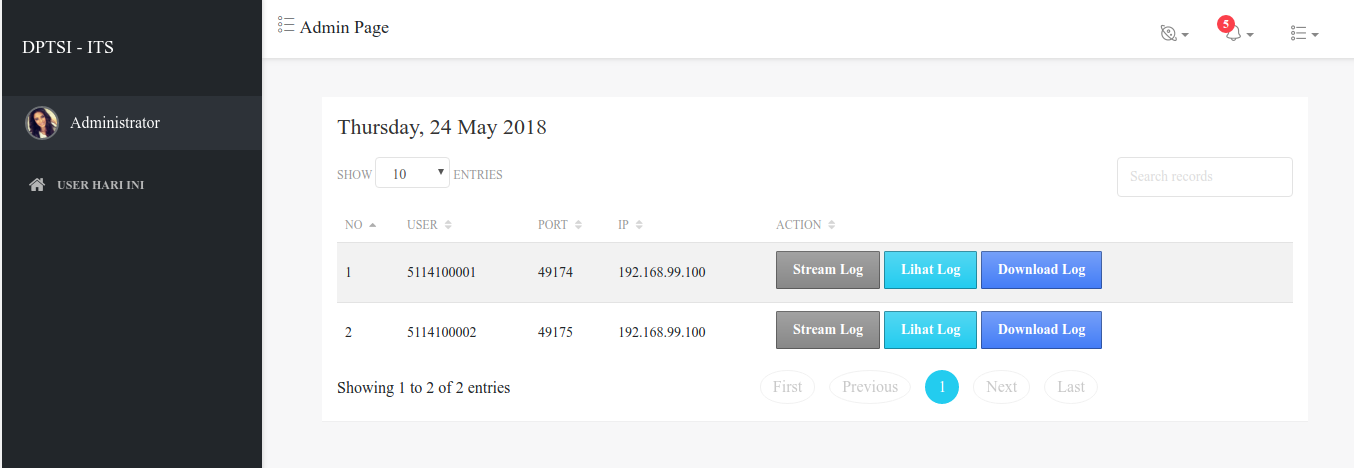
\includegraphics[width=\linewidth]{images/bab4/halamandashboardadmin}
	\caption{Halaman \textit{Login}}
	\label{halamandashboardadmin}
\end{figure}